\section{Experiment 9J: distributed personalized backbone learning}
\label{sec:experiment9j}

\paragraph{Question and protocol.}
Experiment 9J closes the implementation gap left by the centralized summary
experiments: can the unknown-group personalized LPV backbone be learned from
federated aggregate messages, and does it remain useful with partial client
participation? Ten development fleets (seeds 196--205) each contain 180 mature
training clients and 30 unseen test clients. Training clients retain their
structured parameter estimates and uncertainty locally. In each communication
round they compute mixture responsibilities and transmit additive precision,
information-vector, and scatter summaries. The server learns the number of
groups from candidates one through six and constructs group centers and
control-aware principal directions from the aggregated moments. Personalized
coordinates and short calibration records never leave a test client.

Fed100, Fed50, and Fed20 sample 100\%, 50\%, or 20\% of clients per round for
30 rounds. They are compared with the established centralized-summary method,
full three-parameter Local identification, and an exact-individual diagnostic.
The progressive policy frozen after Experiment 9H uses rank one after 0.75~s and
rank two after 1.25~s. Evaluation uses three unseen nonlinear closed-loop
scenarios. Gate A requires a deterministic full-participation rerun to reproduce
the same groups and moments to numerical precision. Gate B limits degradation
relative to Central to 1\% for Fed50 and 2\% for Fed20; improvements do not count
as failures. Gate C requires Fed20 to beat Local at both budgets.

\begin{table}[htbp]
\centering
\caption{Experiment 9J nonlinear tracking RMSE. Percentages compare with Central.}
\label{tab:experiment9j-results}
\begin{tabular}{lrrrr}
\toprule
Method & \multicolumn{2}{c}{0.75 s} & \multicolumn{2}{c}{1.25 s}\\
 & RMSE & vs. Central & RMSE & vs. Central\\
\midrule
Local   & 0.013330 & +23.76\% & 0.007620 & +0.52\%\\
Central & 0.010771 & 0.00\%   & 0.007580 & 0.00\%\\
Fed100  & 0.010771 & 0.00\%   & 0.007580 & 0.00\%\\
Fed50   & 0.010828 & +0.53\%  & 0.007581 & +0.01\%\\
Fed20   & 0.010518 & -2.34\%  & 0.007584 & +0.04\%\\
\bottomrule
\end{tabular}
\end{table}

\begin{table}[htbp]
\centering
\caption{Experiment 9J federated protocol audit (mean per fleet). Payload counts
exclude transport headers and cryptographic overhead.}
\label{tab:experiment9j-communication}
\begin{tabular}{lrrrrr}
\toprule
Method & Groups & ARI & Coverage & Upload & Download\\
\midrule
Fed100 & 3.0 & 1.000 & 1.000 & 1.160 MB & 0.670 MB\\
Fed50  & 3.1 & 0.989 & 1.000 & 0.610 MB & 0.346 MB\\
Fed20  & 3.1 & 0.892 & 0.999 & 0.258 MB & 0.138 MB\\
\bottomrule
\end{tabular}
\end{table}

\begin{figure}[htbp]
\centering
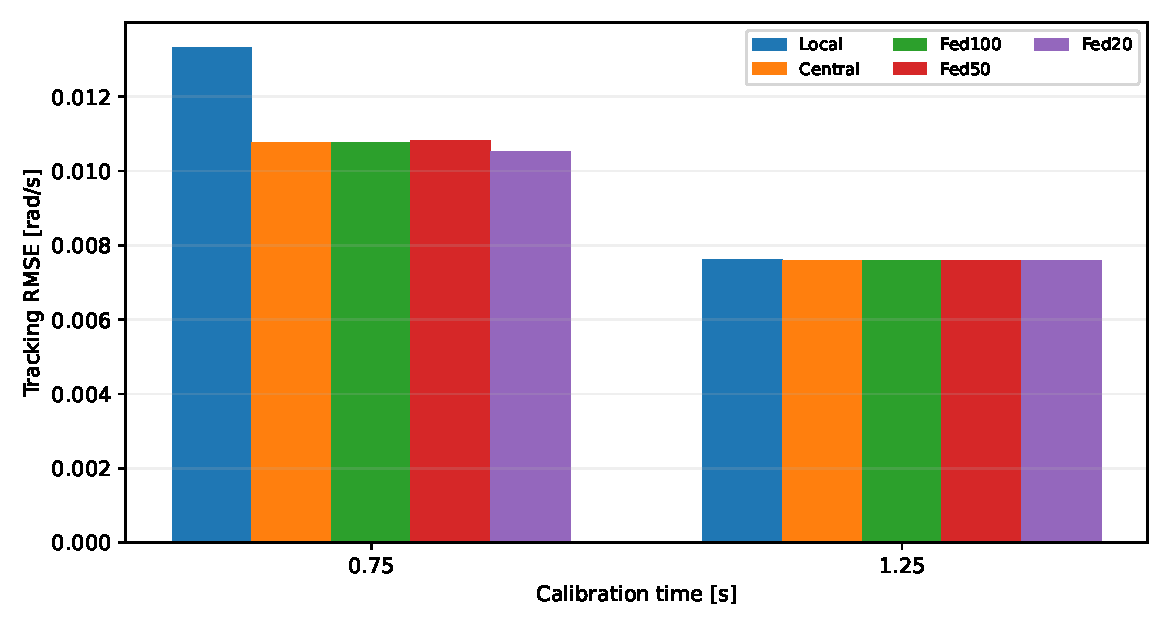
\includegraphics[width=0.84\linewidth]{../results/figures/experiment_9j_distributed_backbone.pdf}
\caption{Distributed shared-backbone learning preserves the cold-start benefit
under partial participation. At 1.25~s the Local estimator has largely caught up.}
\label{fig:experiment9j}
\end{figure}

\paragraph{Result.}
All three gates pass. Fed100 agrees with Central to below
$6\times10^{-8}$\% in tracking, and the independent deterministic aggregation
rerun reproduces the selected group count, means, and covariances to below
$10^{-12}$. Fed50 remains within 0.53\% of Central at both budgets. Fed20 is
2.34\% better at 0.75~s and only 0.04\% worse at 1.25~s. The apparent Fed20
improvement is not claimed as a benefit of dropping clients; it is consistent
with sampling-induced regularization and finite-fleet variation.

Relative to Local, Fed20 improves aggregate tracking by 21.09\% at 0.75~s and
0.47\% at 1.25~s. It wins all ten fleet-wise comparisons at 0.75~s and seven of
ten at 1.25~s. Thus the main operational result is concentrated in cold start:
sharing is valuable when the new client is information limited, while Local
identification catches up as its own excitation becomes adequate. All 2400 fits
converge and all 10800 nonlinear evaluations remain feasible.

\paragraph{FL interpretation and limitations.}
This experiment supplies an explicit federated mechanism rather than merely
calling centralized pooling federated. The server receives only additive
sufficient statistics; raw trajectories, test-client coefficients, and local
calibration records remain local. The aggregation interface is compatible with
secure aggregation, but this simulation does not implement cryptography or
claim resistance to inference from released aggregate models. Communication
figures count 32-bit numerical payloads only. Partial participation is simulated
by random cohorts; stragglers, asynchronous updates, packet loss, and nonrandom
availability remain outside the present scope.

The ten development fleets support the paper mechanism but are not the final
confirmatory evidence. Seeds 206--215 remain untouched for a frozen confirmation
of the complete 9J protocol. Privacy perturbation should subsequently be applied
to these aggregate updates while keeping personalized coordinates local.

\paragraph{Reproducibility.}
The frozen development protocol is in
\path{code/config/experiment_9j.json}. The distributed aggregation implementation
is \path{code/src/federated_lpv/federated_manifold.py}, and the experiment driver
is \path{code/experiments/experiment_9j_distributed_backbone.py}. Aggregate,
seed-level, communication, diagnostic, and provenance records are stored under
\path{results/tables}.
